% Editorially assembled from the preserved September 17 report.
\section{Proof map, experimental provenance, and historical scope}\label{sec:record}
\begin{figure}[tbp]
\centering
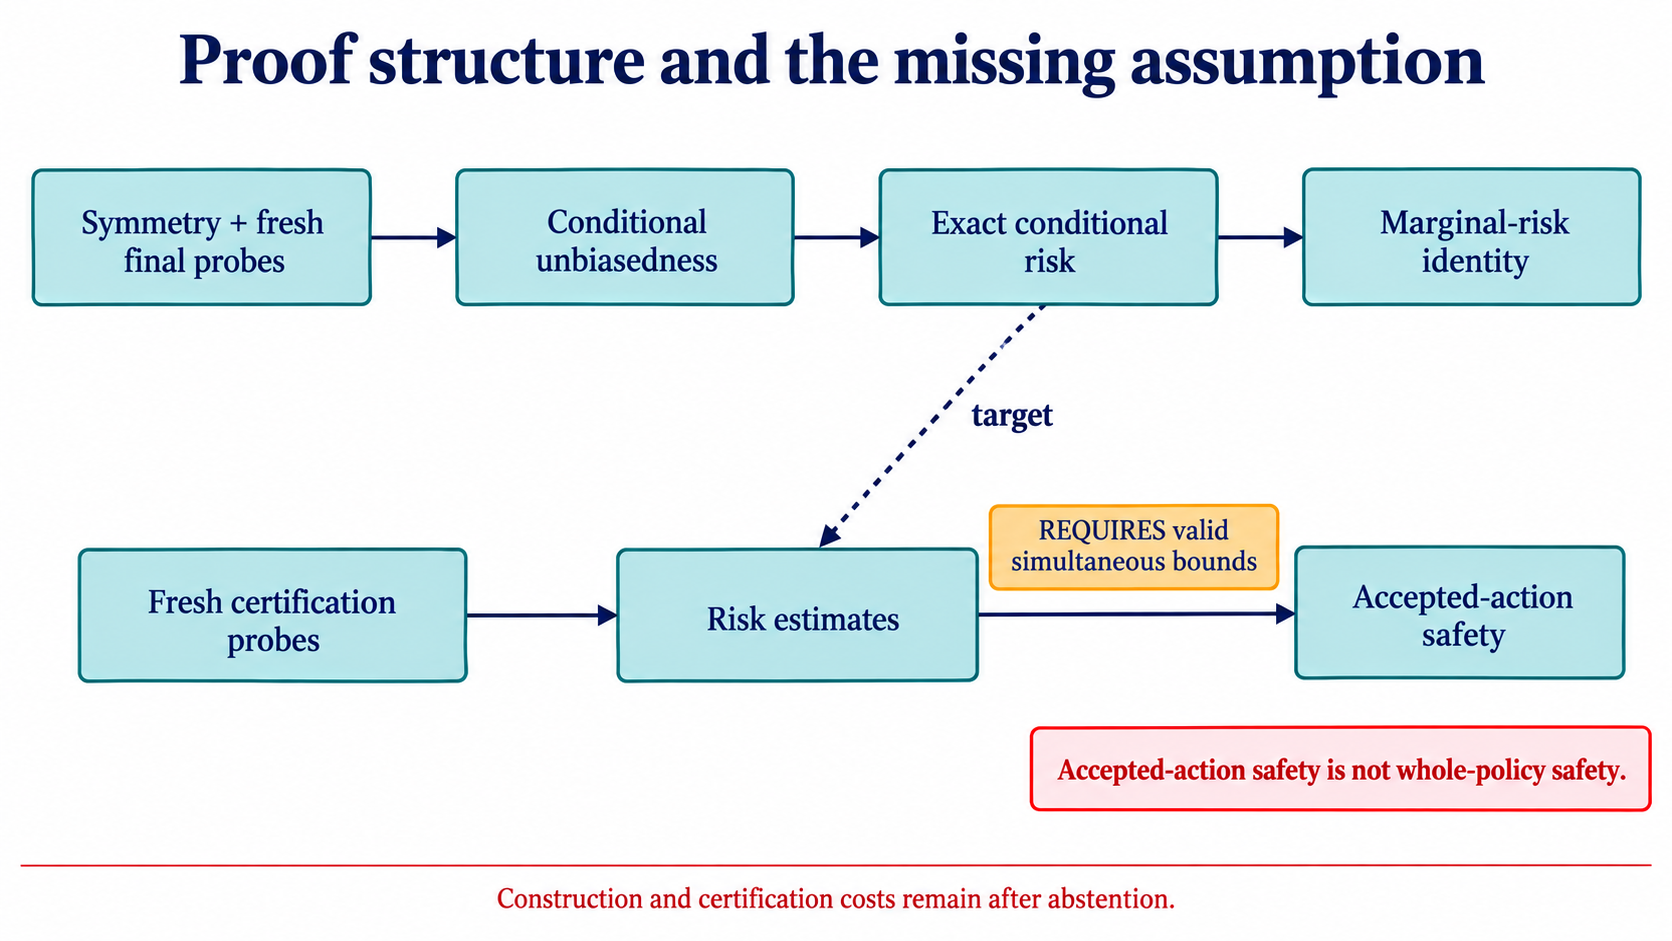
\includegraphics[width=\linewidth]{figures/dependencies.png}
\caption[Proof structure and the missing confidence assumption]{Reading map, not a replacement for the assumptions in the theorems. The upper chain additionally requires orthonormal projectors, positive residual denominators, conditional isotropy, and the specified final-probe law. The lower chain deliberately does \textbf{not} infer valid confidence bounds merely from unbiased risk estimates. GPT-generated conceptual artwork was reviewed for these distinctions; it contains no experimental measurements.}
\label{fig:dependencies}
\end{figure}
\subsection{Development history}
{\small
\begin{longtable}{@{}>{\raggedright\arraybackslash}p{0.2024\linewidth}>{\raggedright\arraybackslash}p{0.2816\linewidth}>{\raggedright\arraybackslash}p{0.3960\linewidth}@{}}
\caption{Historical progression and surviving conclusions}\label{tab:auto6}\\
\toprule
Stage & Question attempted & What survives after the audits \\
\midrule
\endfirsthead
\toprule
Stage & Question attempted & What survives after the audits \\
\midrule
\endhead
Spectral-decay fitting & Can an exponent determine the split? & A visible fit need not predict the unseen tail \\
Multimodel / soft allocation & Can model choice or shrinkage repair fitting? & Model accuracy and allocation risk are different objectives \\
Sequential pilot & Can a detected knee guide the split? & Fresh-probe unbiasedness holds, but pilot commitment costs remain \\
Symmetric / asymmetric guards & Can clipping preserve baseline robustness? & Fixed guards are heuristics; no uniform improvement was established \\
Ideal and realized risk bridges & What objective does allocation actually minimize? & Rank correction alone does not account for subspace leakage \\
Zero-oversampling audit & Why did the finite mean prefer $k+1$? & Rare conditioning failures support oversampling, not a universal +1 rule \\
Phase 1A & Can fresh probes estimate the right risk? & Ordinary sample variance passed the empirical gate \\
Phase 1B & Is the information worth its queries? & Rare-path protection can coexist with harm on most paths \\
Phase 1C / 1D & Can explicit small-budget bounds certify it? & The audited routes are mathematically valid but vacuous \\
Phase 2A / 2B & Does common-probe cancellation help? & It often does empirically; unknown scale still obstructs the audited theorem \\
Phase 2C & Can structural prior information help? & A valid prior gives a conditional finite radius, not free prior knowledge \\
Exploratory two-stage gate & Can cheap pilot features avoid certification cost? & An exact missed direction can survive an extremely sharp visible knee \\
Recovery and consolidation & Which results can be trusted now? & Protocol reruns, corrected moments, checksums, and explicit claim status \\
\bottomrule
\end{longtable}
}
This progression is a sequence of tested distinctions, not a claim that each new method superseded the previous one successfully. Failed hypotheses narrowed the mathematical question.

\subsection{Reproducibility and figure provenance}
September smoke tests overwrote some untracked production CSVs. Recovery reran the original protocols and validated replacement artifacts. Because original overwritten hashes were unavailable, this was \textbf{protocol-based recovery}, not byte-identical restoration. Output-directory isolation, checksum guards, and explicit query counters now protect the maintained experiments. The recovery report remains the authoritative explanation of that incident.


The preceding coordinate audit preserved 156 pre-existing source/result files and passed 225 maintained tests. The quantitative figure builder subsequently passed five focused tests and preserved its seven historical inputs. Those are prior-run records; this editorial revision does not claim to have rerun the full algorithm suite.


This edition makes \textbf{no estimator changes, no threshold changes, no experimental reruns, no new oracle queries, and no new bootstrap samples}. Its local mathematical regression checks test identities and boundary cases; they supplement rather than replace the proofs. The accompanying editorial audit~\cite{project2026} records the actual checks and preserved-file count for this revision.


Uncertainty follows the replication unit. Certification repetitions are clustered within frozen paths, and paths can share orientations. Existing intervals are conditional on that frozen population. They do not estimate unobserved rare-event probabilities or establish universal performance across orientations. No new confidence intervals are claimed for the exploratory Haar/Hessian tables.


The report contains three new GPT-generated \textbf{conceptual structure diagrams} and the three original \textbf{data-rendered quantitative figures}. Their roles are different. Exact assumptions and equations live in the text. Quantitative PNG/SVG plots retain source CSVs and checksums in the validated figure guide~\cite{project2026}. The earlier GPT-polished quantitative companions~\cite{project2026} remain separate presentation assets, not replacements for numerical geometry. New conceptual prompts, edits, and diagram contracts are stored with the diagrams~\cite{project2026}.


\subsection{Manuscript preparation and attribution}
This draft uses the organization of Meyer et al.~\cite{meyer2021} as a
writing reference: early contribution statements, numbered mathematical
results, theory before experiments, and supporting appendices.
It does not copy their prose or imply that their optimality theorem applies
to the adaptive policies studied here.

The source package preserves the detailed September 17 theorem--proof
report and an evidence mapping. It contains all fifteen report-local result
blocks, the spectral corollary, and all six empirical findings, reorganized
into publication-style sections. The capture block is split into two lemmas.
The byline is deliberately neutral pending author confirmation; the
document is a research draft, not a submitted or accepted paper.

Three conceptual figures were generated with an AI image tool and reviewed
for logical labels; they are explanatory illustrations, not data. The three
quantitative figures were rendered from validated frozen numerical records.
Their originals are copied without alteration. AI assistance was used for
editorial restructuring and source preparation; mathematical and scientific
claims require author review before submission.
